\subsection{Descripción del problema.}

\vspace*{0.3cm}

Este problema trata sobre distribuir $N$ productos en $C$ camiones, \textbf{buscando minimizar}
el valor de $C$. Al combinarse los elementos, se obtienen distintos niveles de peligrosidad.
Para minimizar $C$, se debe tener en cuenta que contamos con un umbral de peligrosidad
$M$, \textbf{el cual no debe ser superado por la suma de los niveles de peligrosidad de los
elementos que contiene}.

\vspace*{0.5cm}

\textbf{Ejemplo:}
\begin{itemize}
  \item Dado $M = 7$ y 4 productos $p_1, p_2, p_3$ y $p_4$, con una relación
  de peligrosidad $h_{1,2} = 5, h_{1,3} = 3, h_{1,4} = 4, h_{2,3} = 6, h_{2,4} =
  3$ y $h_{3,4} = 5$, la solución óptima consiste en utilizar 2 camiones: el primero
  transportando $p_1$ y $p_3$ y el segundo transportando $p_2$ y $p_4$.
\end{itemize}


\newpage
\subsection{Desarrollo de la idea y pseudocódigo.}

Para resolver el problema, empezamos utilizando un solo camión e intentamos ubicar
todos los elementos en el mismo. De no ser esto posible, se agrega otro camión y se vuelven
a intentar todas las combinaciones de elementos en los mismos. Si aún asi continuaran sin
caber los $N$ elementos, se agrega un camión más y se vuelve a empezar.

Este proceso continúa, hasta encontrar una cierta cantidad de camiones qie sea capaz de
transportar todos los elementos. Por la estrategia planteada para el problema,
\textbf{la solución encontrada será una solución óptima}.

\vspace*{0.5cm}


\begin{codebox}
\Procname{$\proc{biohazard}(elementos, maximaPeligrosidad)$}
\li $\id{camiones} \gets []$
\li $\proc{agregar}(camiones, camion)$
\li \While $(\neg\proc{backtracking}(camiones, elementos))$
\li     \Do
            $\proc{agregar}(camiones, camion)$
        \End
\li \Return $\id{camiones}$
\end{codebox}


\vspace*{0.5cm}


\begin{codebox}
\Procname{$\proc{backtracking}(camiones, elementos)$}
\li \If $\proc{vacio?}(elementos)$
\li     \Then
            \Return $\const{true}$
        \End
\li $\id{elemento} \gets \proc{dameUno}(elementos)$
\li $\id{elementos} \gets elementos \setminus \{elemento\}$
\li \For $camion \in camiones$
\li     \Do
            \If $\proc{entra?}(elemento, camion)$
\li             \Then
                    $\proc{agregar}(camion, elemento)$
\li                 \If $\proc{backtracking}(camiones, elementos)$
                        \Then
\li                         \Return $\const{true}$
\li                 \Else
\li                     $\proc{borrar}(camion, elemento)$
                    \End
            \End
        \End
\li $\id{elementos} \gets elementos \cup \{elemento\}$
\li \Return $\const{false}$
\end{codebox}



\newpage
\subsection{Análisis de complejidad.}

\vspace*{0.3cm}

\textbf{completar!}


\newpage
\subsection{Experimentación y gráficos.}

\vspace*{0.3cm}

\subsubsection{Test 1 - benchmark caso aleatorio}

(ver \verb|info.3.dat|) \medskip

En este test, tenemos $n$ elementos en cada instancia, con $n$ inicializado en 1 e incrementándose
también en 1 hasta alcanzar 20 y un umbral $m$ de peligrosidad, que se inicializa en 2 y se incrementa
en 2 en cada instancia, hasta alcanzar el valor 40.

Para cada instancia, se toma el \textbf{valor mínimo} de cantidad de ciclos luego de \textbf{20 corridas}.

\vspace*{0.5cm}

% \begin{figure}[h]
%   \begin{center}
%     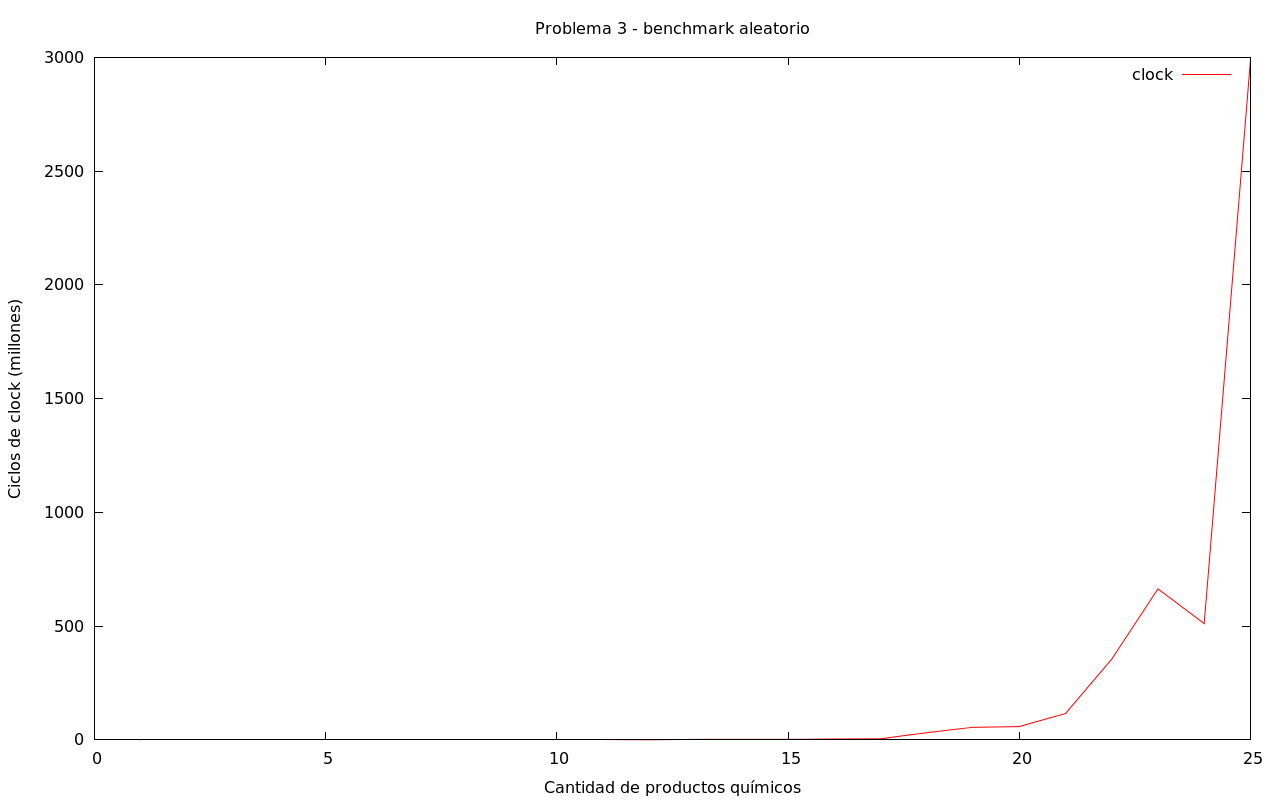
\includegraphics[scale=0.35]{imagenes/grafico-3.png}
%   \end{center}
% \end{figure}

\vspace*{0.5cm}

En este gráfico podemos apreciar que el comportamiento del algoritmo es
sumamente aleatorio en el caso promedio. Esto se debe a la naturaleza poco
predecible del mismo, ya que en base a cómo sean los valores de entrada, las
podas se realizan en momentos diferentes.


\newpage
\subsubsection{Test 2 - benchmark del peor caso}

(ver \verb|info.3.peor.dat|) \medskip

\underline{\textbf{NOTA:}} para el peor caso redujimos la cantidad de instancias a 16 por fines prácticos, dada la complejidad
del algoritmo y el tiempo de ejecución requerido para finalizar más instancias. \medskip

En este test, tenemos $n$ elementos en cada instancia, con $n$ inicializado en 1 e incrementándose
también en 1 hasta alcanzar 16 y un umbral $m$ de peligrosidad, que se mantiene constante en 0 para todas las
instancias.

Para cada instancia, se toma el \textbf{valor mínimo} de cantidad de ciclos luego de \textbf{16 corridas}.

\vspace*{0.5cm}

% \begin{figure}[h]
%   \begin{center}
%     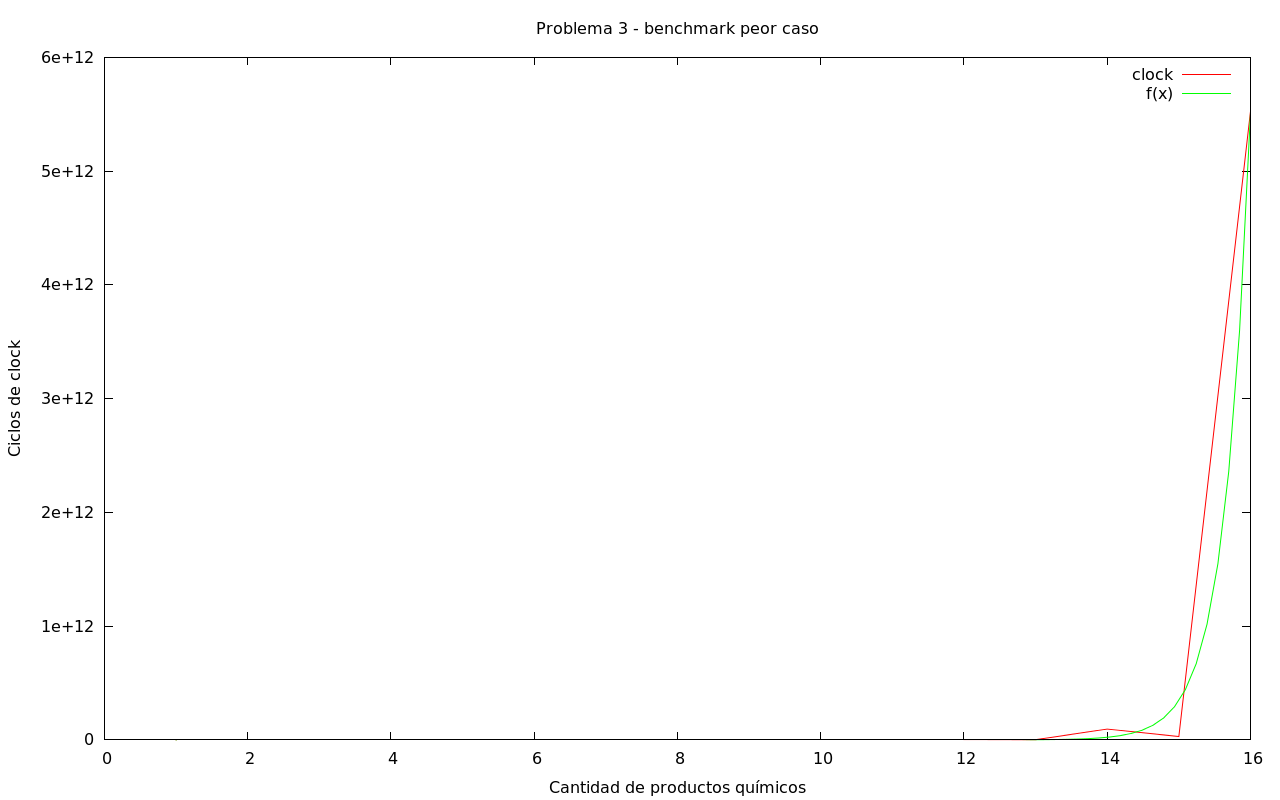
\includegraphics[scale=0.35]{imagenes/grafico-3-peor.png}
%   \end{center}
% \end{figure}

\vspace*{0.5cm}

En este gráfico podemos apreciar que a partir de los 10 elementos, el
crecimiento de la cantidad de ciclos de clocks necesarios para completar las
instancias crece exponencialmente, llegando a un pico de casi 6 billones de
ciclos de clock.


\newpage
\subsubsection{Test 3 - benchmark del mejor caso}

(ver \verb|info.3.mejor.dat|) \medskip

En este test, tenemos $n$ elementos en cada instancia, con $n$ inicializado en 1 e incrementándose
también en 1 hasta alcanzar 20 y un umbral $m$ de peligrosidad, que se inicializa en 1000000 y se incrementa
también de a 1000000 en cada instancia, hasta alcanzar el valor 20000000.

Para cada instancia, se toma el \textbf{valor mínimo} de cantidad de ciclos luego de \textbf{20 corridas}.


% \begin{figure}[h]
%   \begin{center}
%     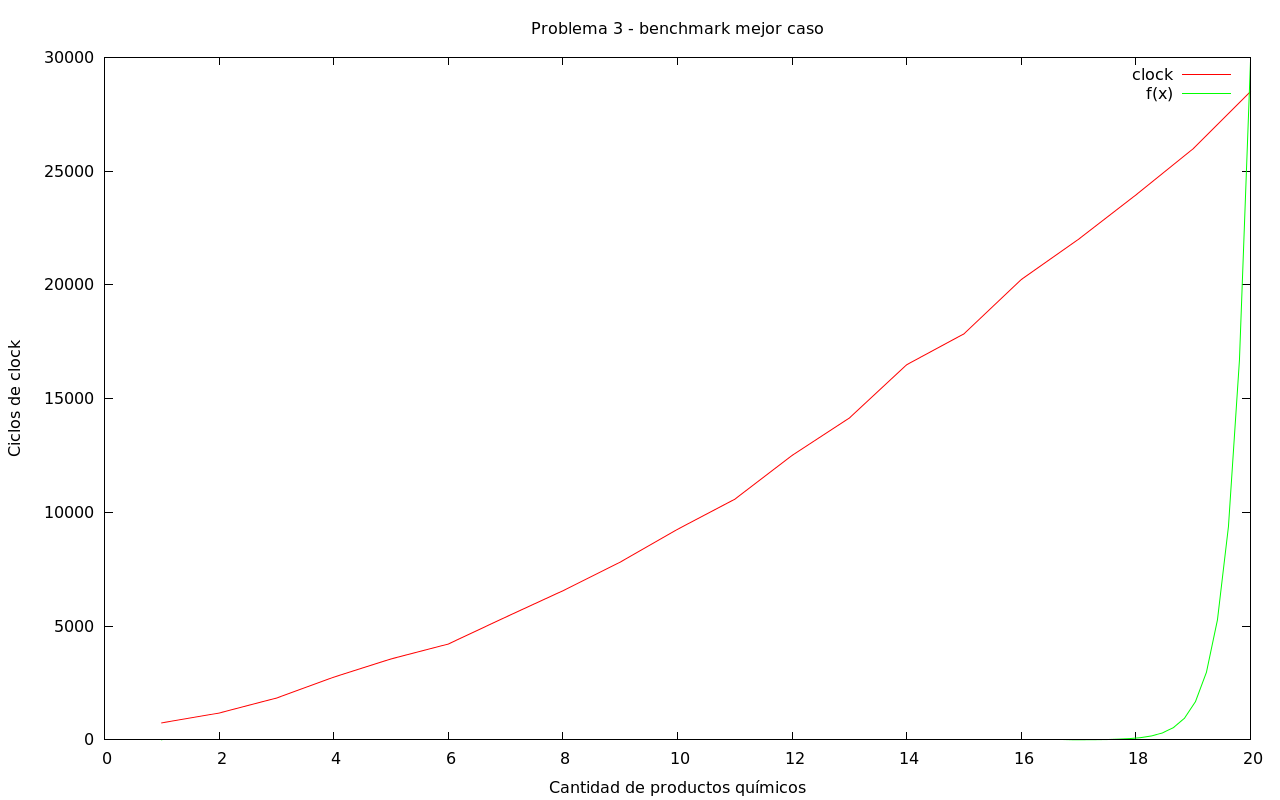
\includegraphics[scale=0.35]{imagenes/grafico-3-mejor.png}
%   \end{center}
% \end{figure}


En este gráfico podemos apreciar que el algoritmo, tiene un comportamieno
muy veloz en comparación contra instancias aleatorias o de peor caso. Esto
se debe a que el mismo se reduce a realizar una pequeña serie de sumas en el
caso de que todos los elementos entren en un solo camión.
